%Este trabalho está licenciado sob a Licença Atribuição-CompartilhaIgual 4.0 Internacional Creative Commons. Para visualizar uma cópia desta licença, visite http://creativecommons.org/licenses/by-sa/4.0/deed.pt_BR ou mande uma carta para Creative Commons, PO Box 1866, Mountain View, CA 94042, USA.

\chapter{Interpolação}\label{cap_interp}
\thispagestyle{fancy}

Neste capítulo, estudamos a \hl{resolução de problemas de interpolação} da forma: dados uma família de $n$ funções reais
\begin{equation}\hleq
  \mathcal{F} = \{f_1(x), f_2(x), \dotsc, f_n(x)\}
\end{equation}
e um conjunto de $n$ pontos $\{(x_i, y_i)\}_{i=1}^n$, com $x_i\neq x_j$ se $i\neq j$, encontrar a \emph{função interpoladora}
\begin{equation}\hleq
  f(x) = c_1f_1(x) + c_2f_2(x) + \cdots + c_nf_n(x),
\end{equation}
tal que
\begin{equation}\hleq
  y_i = f(x_i),\quad i=1, 2, \ldots, n.
\end{equation}

\section{Interpolação Polinomial}\label{cap_interp_sec_interpoli}

\hl{Dado um conjunto de $n$ pontos $\{(x_i, y_i)\}_{i=1}^n$, o problema de interpolação consiste em encontrar o polinômio\footnote{Chamado de \emph{polinômio interpolador}.} de grau $n-1$}
\begin{equation}\label{cap_interp_sec_interpoli:eq:interpoli_poli}\hleq
  p(x) = p_1x^{n-1} + p_2x^{n-2} + \cdots + p_{n-1}x + p_n
\end{equation}
tal que
\begin{equation}\label{cap_interp_sec_interpoli:eq:interpoli_conds}\hleq
  y_i = p(x_i),
\end{equation}
para todo $i=1, 2, \dotsc, n$.

Das condições \eqref{cap_interp_sec_interpoli:eq:interpoli_poli}, temos
\begin{equation}
  \begin{aligned}\label{cap_interp_sec_interpoli:eq:interpoli_sis}
    p_1x_1^{n-1} + p_2x_1^{n-2} + \cdots + p_{n-1}x_1 + p_n &= y_1 \\
    p_1x_2^{n-1} + p_2x_2^{n-2} + \cdots + p_{n-1}x_2 + p_n &= y_2 \\
    &\vdots \\
    p_1x_n^{n-1} + p_2x_n^{n-2} + \cdots + p_{n-1}x_n + p_n &= y_n.
  \end{aligned}
\end{equation}
Isto é, \hl{os coeficientes do \emph{polinômio interpolador} {\eqref{cap_interp_sec_interpoli:eq:interpoli_poli}} satisfazem o sistema linear}
\begin{equation}\hleq
  A\pmb{p} = \pmb{y},
\end{equation}
onde $A$ é a \emph{matriz de Vandermonde}{\vandermonde}
\begin{equation}\hleq
  A =
  \begin{bmatrix}
    x_1^{n-1} & x_1^{n-2} & \ldots & x_1 & 1 \\
    x_2^{n-1} & x_2^{n-2} & \ldots & x_2 & 1 \\
    \vdots  & \vdots  & \vdots  & \vdots & \vdots \\
    x_n^{n-1} & x_n^{n-2} & \ldots & x_n & 1
  \end{bmatrix},
\end{equation}
$\pmb{p} = (p_1, p_2, \ldots, p_n)$ é o \emph{vetor das incógnitas} e $\pmb{y} = (y_1, y_2, \ldots, y_n)$ é o \emph{vetor dos termos constantes}.

\begin{ex}\label{cap_interp_sec_interpoli:ex:interpoli_intro}
  Consideramos o problema de encontrar o polinômio interpolador do conjunto de pontos $\{(-1,~-1), (0,~1), (1,~1/2)\}$. Como temos 3 pontos, o polinômio tem grau 2 e pode ser escrito na forma
  \begin{equation}
    p(x) = p_1x^2 + p_2x + p_3.
  \end{equation}
  Seguindo a abordagem acima, temos $\pmb{p}=(p_1, p_2, p_3)$, $\pmb{x} = (-1, 0, 1)$, $\pmb{y}=(-1, 1, 1/2)$ e
  \begin{equation}
    A =
    \begin{bmatrix}
      x_1^2 & x_1 & 1\\
      x_2^2 & x_2 & 1\\
      x_3^2 & x_3 & 1
    \end{bmatrix}.
  \end{equation}
  Então, resolvendo $A\pmb{p} = \pmb{y}$, obtemos o polinômio interpolador
  \begin{equation}
    p(x) = -1,25x^2 + 0,75x + 1.
  \end{equation}
A Figura \ref{cap_interp_sec_interpoli:fig:interpoli_intro} mostra os esboços do polinômio interpolador $p(x)$ e  dos pontos dados.

\begin{figure}[H]
  \centering
  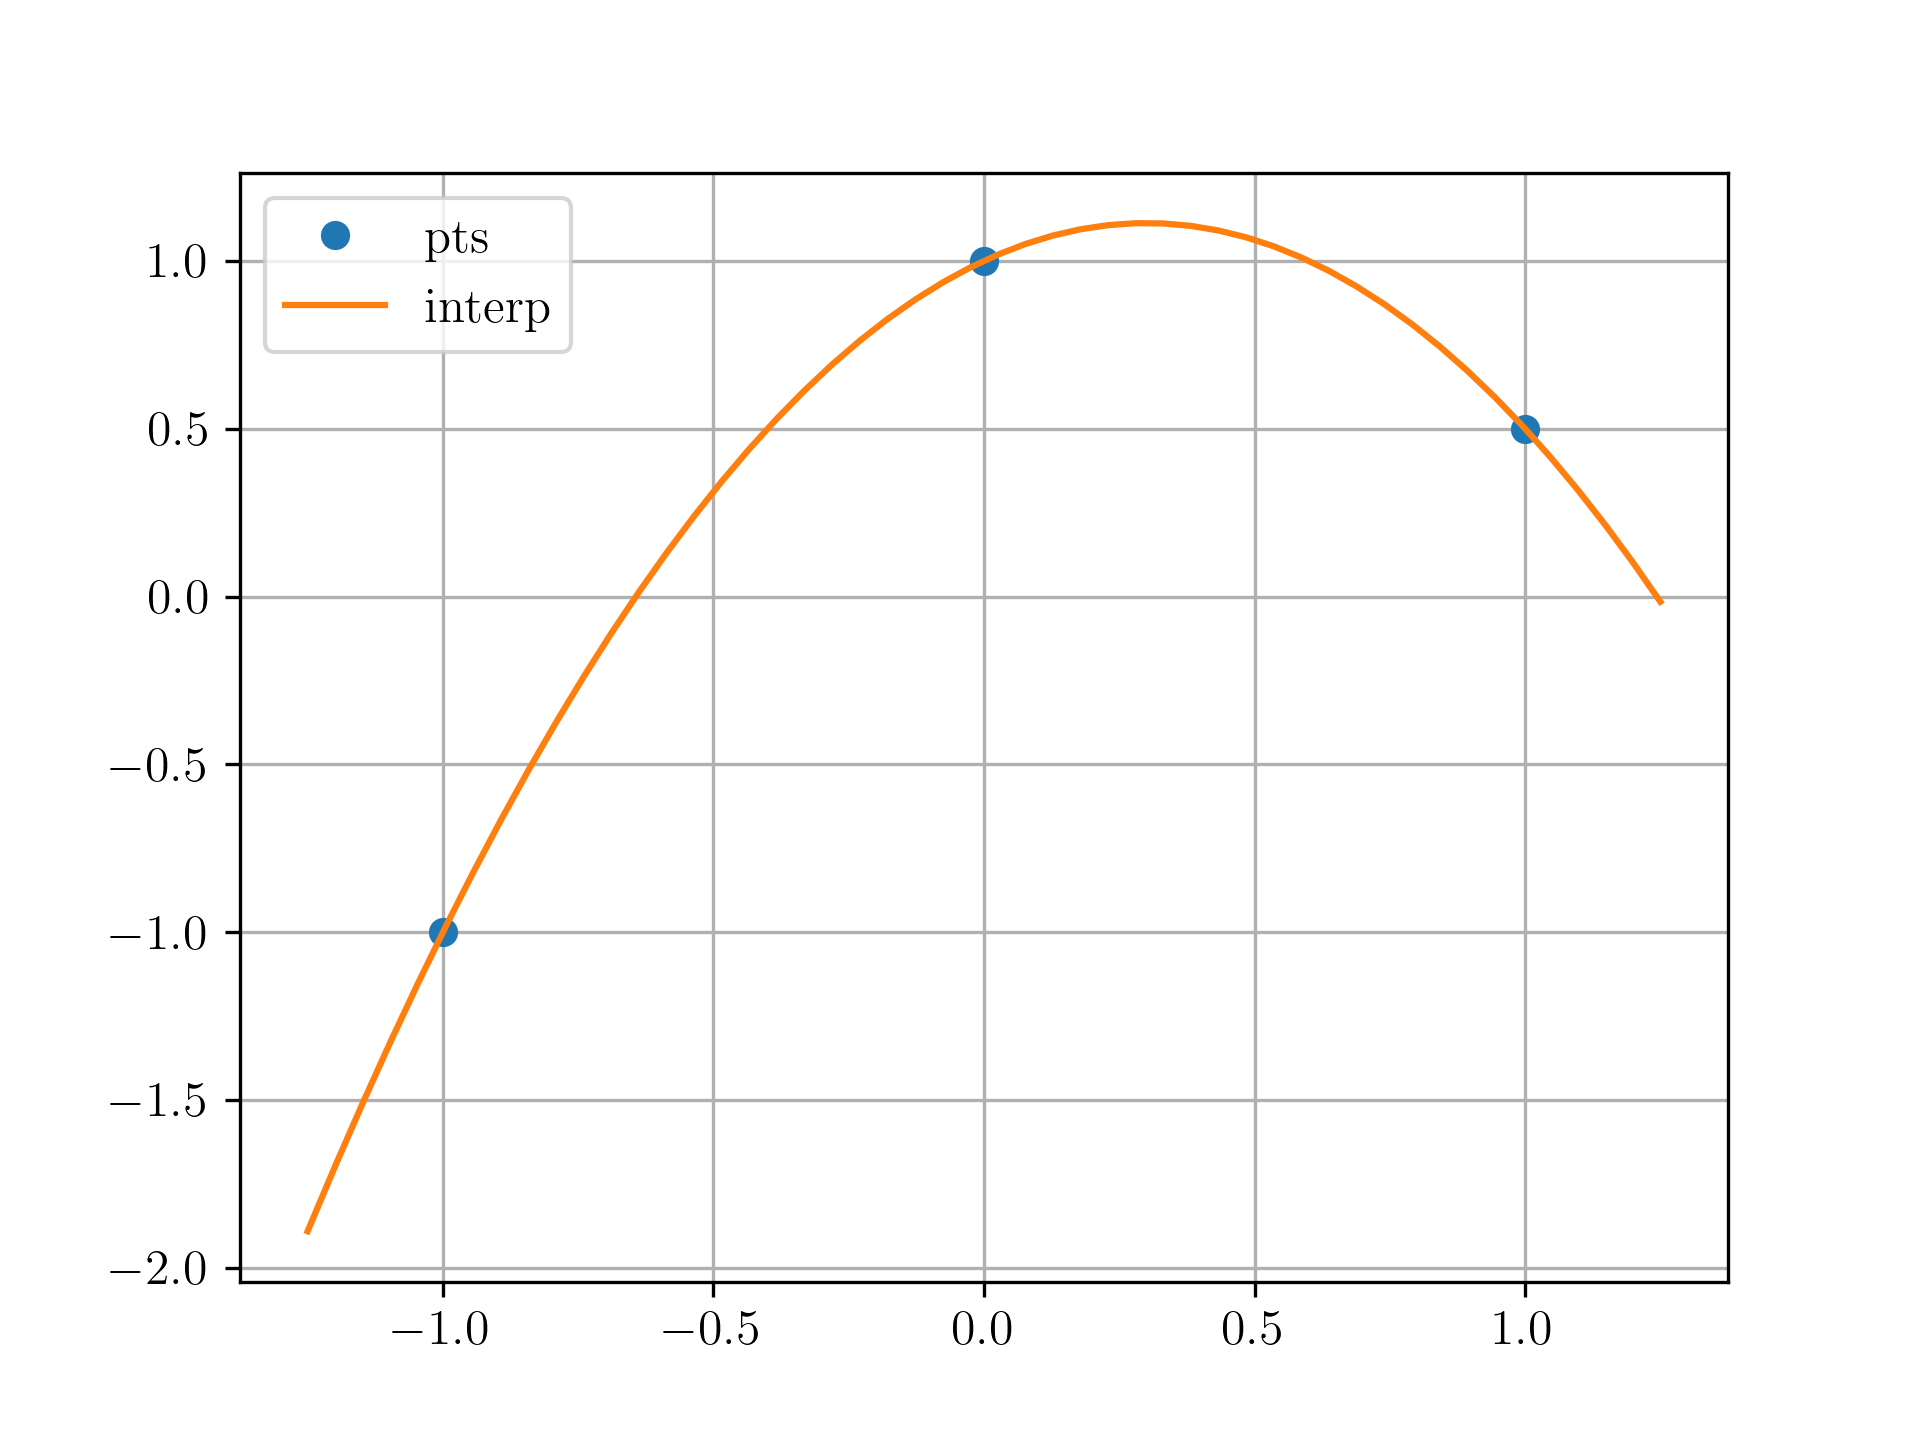
\includegraphics[width=0.7\textwidth]{./cap_interp/dados/fig_poliInterp/fig}
  \caption{Esboço do polinômio interpolador referente ao Exemplo \ref{cap_interp_sec_interpoli:ex:interpoli_intro}.}
  \label{cap_interp_sec_interpoli:fig:interpoli_intro}
\end{figure}

\begin{lstlisting}[caption=poliInterp.py]
import numpy as np
import numpy.linalg as npla

def poliInterp(x, y):
    # num. pts
    n = x.size
    # Vandermonde
    A = np.empty((n,n))
    for j in range(n):
        A[:,j] = x**(n-1-j)
    # coefs
    p = npla.solve(A, y)
    return p

# exemplo
x = np.array([-1., 0, 1])
y = np.array([-1., 1, 1/2])

# poli interp
p = poliInterp(x, y)

# verificação
print(np.polyval(p, x))
\end{lstlisting}
\end{ex}

\subsection{Exercícios}

\begin{exer}
  Obtenha o polinômio interpolador do conjunto de pontos $\{(-1, -1), (-0.5, 1), (1, 2)\}$.
\end{exer}
\begin{resp}
  $-1,\bar{6}x^2 + 1.5x + 2.1\bar{6}$
\end{resp}

\begin{exer}
  Obtenha o polinômio interpolador do conjunto de pontos $\{(-1, -1), (0, 1), (1, 1/2), (2, 1)\}$.
\end{exer}
\begin{resp}
  $0,58\bar{3}x^3 - 1,25x^2 + 0,1\bar{6}x + 1$. 
\end{resp}

\begin{exer}
  Obtenha o polinômio interpolador do conjunto de pontos $\{(-1,~-1), (0,~1), (1,~1/2), (2,~1), (2.5, 1)\}$.
\end{exer}
\begin{resp}
  $-0.26190476x^4  1.10714286x^3 -0.98809524x^2 -0.35714286x  1$.  
\end{resp}

\begin{exer}
  Considere a matriz de Vandermonde $V = [\pmb{x}^{n-j}]_{j=1}^{n}$, com $\pmb{x} = (x_1, x_2, \dotsc, x_n)$, sendo $x_i = (i-1)h$, $h=0.1$ e $i = 1, 2, \dotsc, n$. Compute o número de condicionamento de $V$ para $n=5, 10, 100$. De que forma os resultados obtidos impactam no problema de interpolação polinomial?
\end{exer}
\begin{resp}
  \begin{tabular}{ll}
    $n$ & $\kappa(V)$\\\hline
    $5$ & $1.03\E+4$\\
    $10$ & $2.57\E+7$\\
    $100$ & $9.11\E+109$\\\hline
  \end{tabular}
\end{resp}

\begin{exer}
  Aproxime a função $f(x) = \cos(x)$ por um polinômio interpolador $p$ no intervalo $[0, \pi]$. Escolhas pontos nesse intervalo de forma a obter $p$ que aproxime $f$ com boa precisão gráfica.
\end{exer}
\begin{resp}
  Dica: use os pontos $x_i = (i-1)\frac{\pi}{4}$, $i=1,2,3,4$.
\end{resp}

\section{Interpolação de Lagrange}\label{cap_interp_sec_lagrange}

\hl{Interpolação de Lagrange{\lagrange} é uma técnica para a computação do polinômio interpolador $p(x)$ de um conjunto de pontos $\{(x_i, y_i)\}_{i=1}^n$ dados}. A ideia consiste em escrever o polinômio interpolador na forma
\begin{subequations}\hleq
  \begin{align}
    p(x) &= \sum_{i=1}^n y_iL_i(x)\\
         &= y_1L_1(x) + y_2L_2(x) + \cdots + y_nL_n(x),
  \end{align}
\end{subequations}
onde $L_i(x)$ é chamado de $i$-ésimo polinômio de Lagrange e é definido como o polinômio de grau $n-1$ que satisfaz
\begin{equation}\hleq
  L_i(x_j) = \left\{
    \begin{array}{ll}
      1 &, i=j\\
      0 &, i\neq j
    \end{array}
\right.
\end{equation}
Mais especificamente, temos que \hl{$L_i(x)$ tem raízes $\{x_1, \ldots, x_{i-1}, x_{i+1}, \ldots, x_n\}$} e, portanto, pode ser decomposto na forma
\begin{subequations}
  \begin{align}
    L_i(x) &= c_i\prod_{\overset{j=1}{j\neq i}}^n (x-x_j)\\
           &= c_i(x-x_1)\cdots(x-x_{i-1})(x-x_i)\cdots(x-x_n).
  \end{align}
\end{subequations}
Além disso, como $L_i(x_i) = 1$, temos
\begin{equation}
  c_i = \frac{1}{\displaystyle\prod_{\overset{j=1}{j\neq i}}^n (x_i-x_j)}.
\end{equation}
Assim sendo, podemos concluir que
\begin{subequations}\hleq
  \begin{align}
    L_i(x) &= \prod_{\overset{j=1}{j\neq i}}^n \frac{x-x_j}{x_i-x_j}\\
           &= \frac{(x-x_1)\cdots(x-x_{i-1})(x-x_{i+1})\cdots(x-x_n)}{(x_i-x_1)\cdots(x_i-x_{i-1})(x_i-x_{i+1})\cdots(x_i-x_n)}.
  \end{align}
\end{subequations}

\begin{ex}
  Consideramos o problema de encontrar o polinômio interpolador do conjunto de pontos $\{(-1, -1), (0, 1), (1, 1/2)\}$. Como temos 3 pontos, o polinômio tem grau 2 e pode ser escrito na seguinte forma de Lagrange
  \begin{equation}
    p(x) = y_1L_1(x) + y_2L_2(x) + y_3L_3(x),
  \end{equation}
  onde $y_1 = -1$, $y_2 = 1$ e $y_3 = 1/2$. Os polinômios de Lagrange são dados por
  \begin{align}
    L_1(x) &= \frac{(x-x_2)(x-x_3)}{(x_1-x_2)(x_1-x_3)} \\
           &= \frac{1}{2}x^2 - \frac{1}{2}x,\\
    L_2(x) &= \frac{(x-x_1)(x-x_3)}{(x_2-x_1)(x_2-x_3)} \\
           &= -x^2 + 1,\\
    L_3(x) &= \frac{(x-x_1)(x-x_2)}{(x_3-x_1)(x_3-x_2)} \\
           &= \frac{1}{2}x^2 + \frac{1}{2}x.\\
  \end{align}
  E, então, temos o polinômio interpolador
  \begin{equation}
    p(x) = -1,25x^2 + 0,75x + 1.
  \end{equation}

\begin{lstlisting}[caption=poliLagrange.py]
import numpy as np
from itertools import chain

def poliLagrange(x, xpts, ypts):
    # num. pts
    n = xpts.size
    # Lagrange poli
    L = np.ones((n,x.size))
    y = 0
    for i in range(n):
        for j in chain(range(i),range(i+1,n)):
            L[i] *= (x-xpts[j])/(xpts[i]-xpts[j])
        y += ypts[i] * L[i]
    return y

# exemplo
xpts = np.array([-1., 0, 1])
ypts = np.array([-1., 1, 1/2])

# verificação
x = xpts.copy()
print(poliLagrange(x, xpts, ypts))
\end{lstlisting}
\end{ex}

\subsection{Aproximação de Funções}

Polinômio interpoladores podem ser usados para a aproximação de funções. \hl{Podemos aproximar uma dada função $f$ pelo polinômio interpolador de um conjunto de pontos selecionados $\{(x_i, y_i=f(x_i))\}_{i=1}^n$}. De fato, o seguinte teorema nos fornece uma estimativa para o erro de uma tal interpolação.

\begin{teo}\normalfont{(\hl{Teorema de Lagrange}.)}\label{cap_interp_sec_lagrange:teo:lagrange}
  Sejam dados uma função $f\in C^{n+1}([a, b])$ e $n$ pontos $\{x_i\}_{i=1}^n\subset [a, b]$. Então, o polinômio interpolador do conjunto de pontos $\{x_i, y_i=f(x_i)\}_{i=1}^n$ satisfaz
  \begin{equation}\hleq
    f(x) = p(x) + \frac{f^{(n+1)}(\xi)}{(n+1)!}\prod_{i=1}^n(x-x_i).
  \end{equation}
\end{teo}
\begin{dem}

  [[tag:construcao]]

\end{dem}

\begin{ex}\label{cap_interp_sec_lagrange:ex:interpoli_aprox}
  Consideramos o problema de aproximar $f(x) = \sen(x)$ pelo polinômio interpolador do conjunto de pontos $x_1=0$, $x_2=\pi/2$ e $x_3=\pi$. I.e., queremos determinar o polinômio $p(x)$ de grau $2$ que interpola os pontos $\{(0, 0),~(\pi/2, 1),~(\pi, 0)\}$. Usando a técnica de Lagrange, obtemos
  \begin{equation}
    p(x) = -0,41x^2 + 1,3x,
  \end{equation}
com seus coeficientes arredondados para dois dígitos significativos. A Figura \ref{fig:interpoli_aprox} mostra os esboços da função $f(x)=\sen(x)$, dos pontos dados e do polinômio interpolador $p(x)$.

\begin{figure}[H]
  \centering
  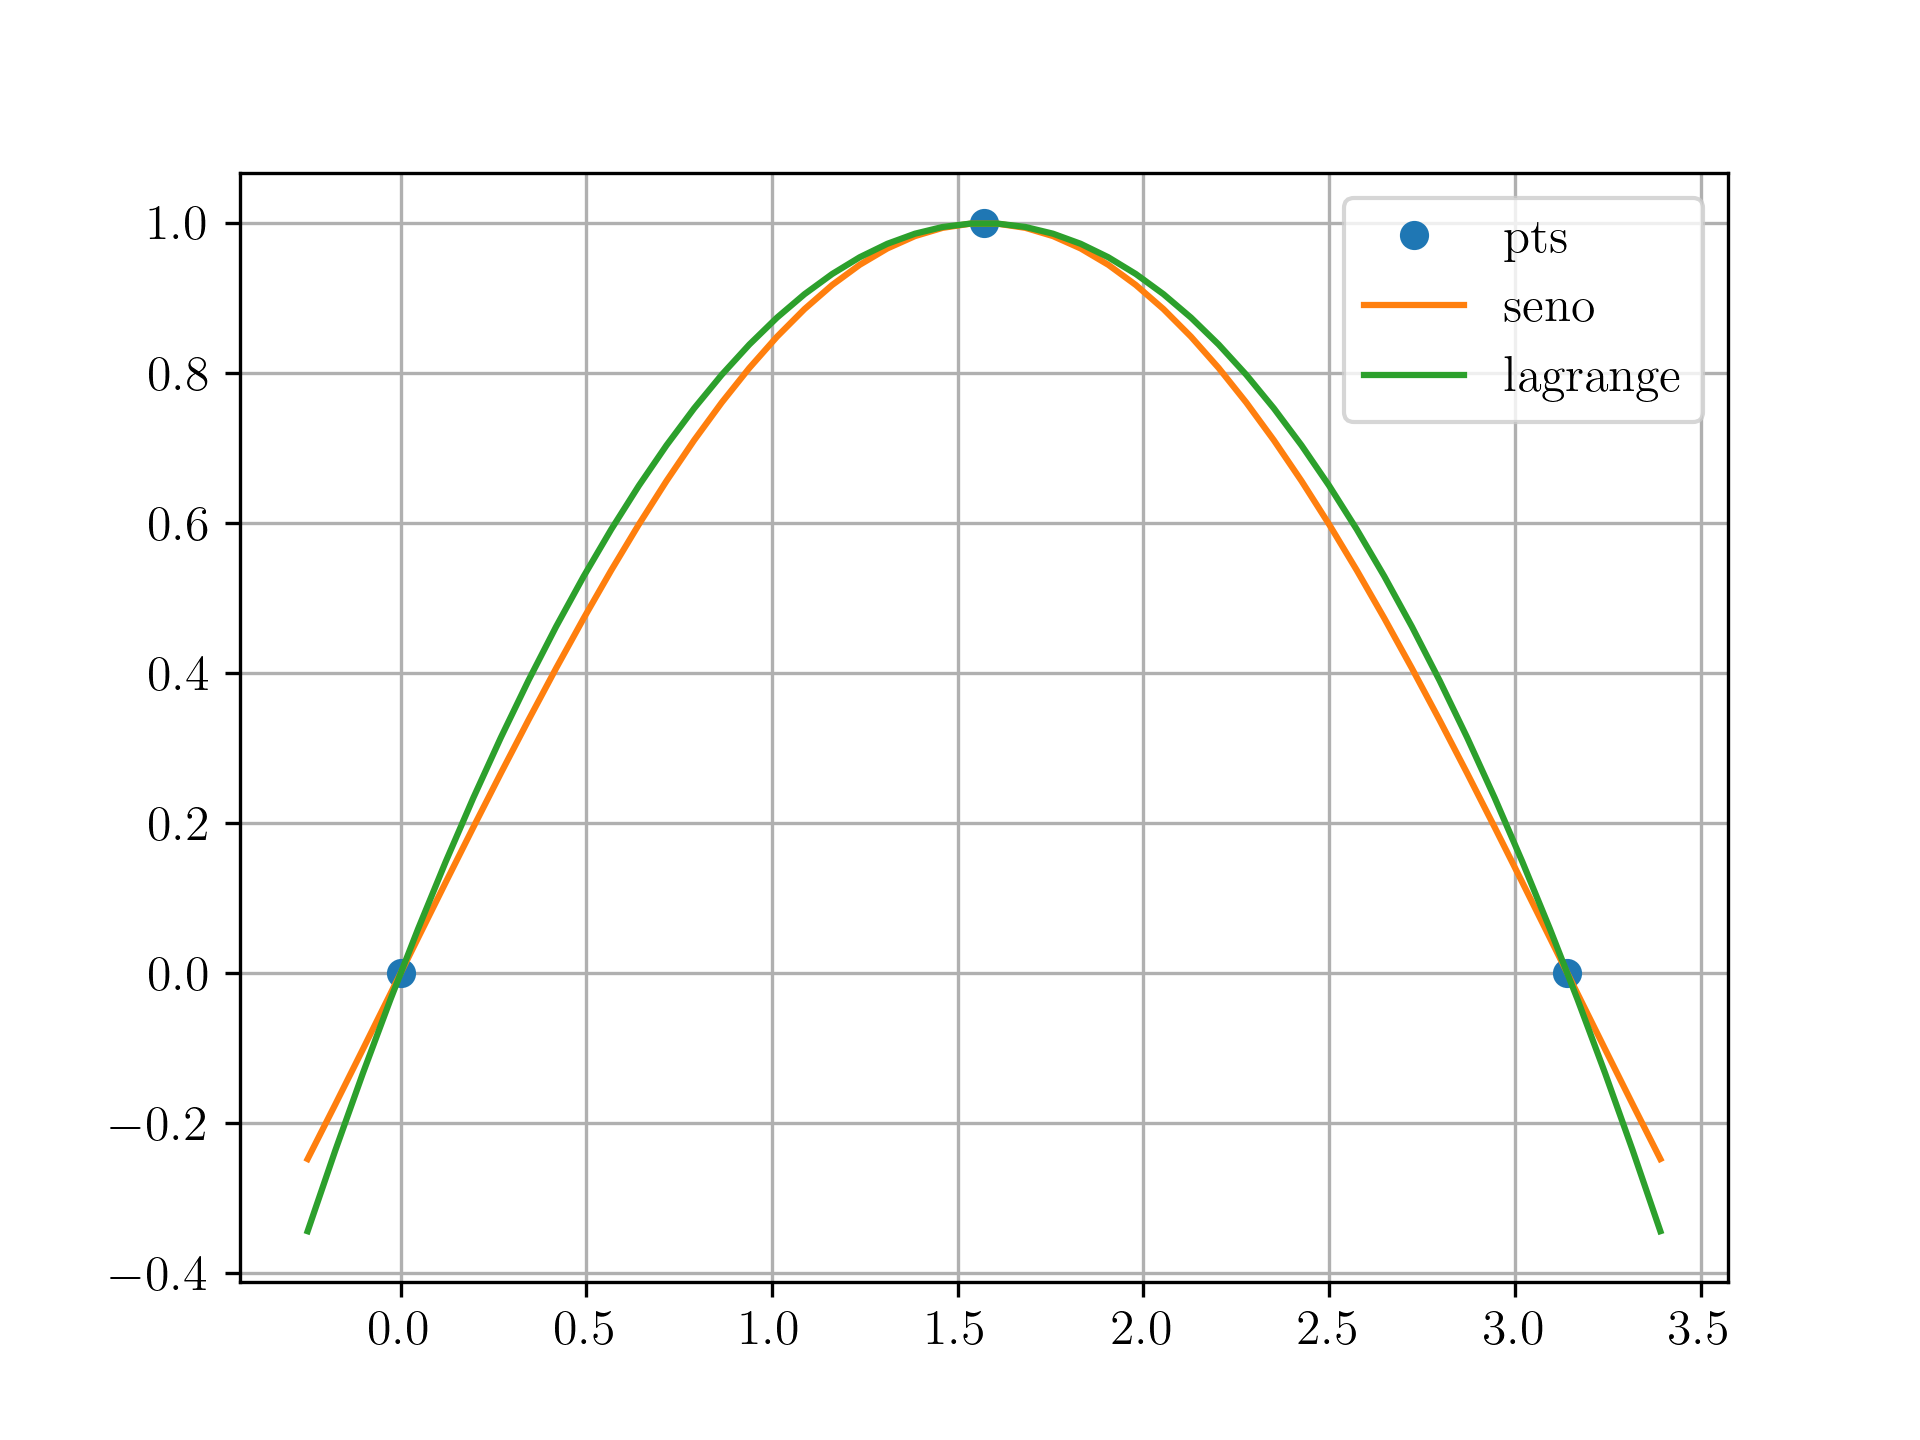
\includegraphics[width=0.7\textwidth]{./cap_interp/dados/fig_poliLagrange/fig}
  \caption{Esboços dos gráficos da função, dos pontos e do polinômio interpolador computado no Exemplo \ref{cap_interp_sec_lagrange:ex:interpoli_aprox}.}
  \label{cap_interp_sec_lagrange:fig:interpoli_aprox}
\end{figure}

\begin{lstlisting}
x = np.array([0, np.pi/2, np.pi])
f = lambda x: np.sin(x)
poli = lagrange(x, f(x))
\end{lstlisting}
\end{ex}

\subsection*{Exercícios}

\begin{exer}
  Use a técnica de Lagrange para obter o polinômio interpolador do conjunto de pontos $\{(-1, -1), (-0.5, 1), (1, 2)\}$.
\end{exer}
\begin{resp}
  $-1,\bar{6}x^2 + 1.5x + 2.1\bar{6}$
\end{resp}

\begin{exer}
  Use a técnica de Lagrange para obter o polinômio interpolador do conjunto de pontos $\{(-1, -1), (0, 1), (1, 1/2), (2, 1)\}$.
\end{exer}
\begin{resp}
  $0,58\bar{3}x^3 - 1,25x^2 + 0,1\bar{6}x + 1$. 
\end{resp}

\begin{exer}
  Use a técnica de Lagrange para obter o polinômio interpolador do conjunto de pontos $\{(-1,~-1), (0,~1), (1,~1/2), (2,~1), (2.5, 1)\}$.
\end{exer}
\begin{resp}
  $-0.26190476x^4  1.10714286x^3 -0.98809524x^2 -0.35714286x  1$.  
\end{resp}

\begin{exer}
  Use a técnica de interpolação de Lagrange para encontrar o polinômio interpolador que aproxima a função$f(x)=e^{x}$ pelos pontos $x_1=0$, $x_2=1$, $x_3=1,5$ e $x_4=2$.
\end{exer}
\begin{resp}
$0,54x^3 - 0,15x^2 + 1,3x + 1$.
\end{resp}

\begin{exer}
  Use a técnica de Lagrange para aproximar a função $f(x) = \cos(x)$ por um polinômio interpolador $p$ no intervalo $[0, \pi]$. Escolha pontos de forma a obter $p$ que aproxime $f$ com boa precisão gráfica.
\end{exer}
\begin{resp}
  Dica: use os pontos $x_i = (i-1)\frac{\pi}{4}$, $i=1,2,3,4$.
\end{resp}

\section{Diferenças Divididas de Newton}\label{cap_interp_sec_difdiv}

Dado um conjunto de pontos $\{(x_i, y_i)\}_{i=1}^n$, o \hl{\emph{Método das Diferenças Divididas de Newton}}{\newton} busca determinar o \hl{polinômio interpolador da forma}
\begin{equation}\hleq
  \begin{aligned}
    p(x) &= a_1 + a_2(x-x_1) \\
    &+ a_3(x-x_1)(x-x_2)\\
    &+ \cdots + a_{n}(x-x_1) \cdots (x-x_{n-1}).
  \end{aligned}
\end{equation}
Por uma abordagem direta, temos que $p(x_i)=y_i$, $i=1, 2, \dotsc, n$, o que nos leva ao seguinte sistema triangular inferior
\begin{subequations}
  \begin{align}
    a_1 &= y_1, \\
    a_1 + a_2(x_2-x_1) &= y_2, \\
    a_1 + a_2(x_3-x_1) + a_3(x_3-x_1)(x_3-x_2) &= y_3, \\
        &\vdots\\
    a_1 + a_2(x_n-x_1) + \cdots + a_{n}(x_n-x_1)\cdot\cdots\cdot(x_n-x_{n-1}) &= y_n.
  \end{align}
\end{subequations}
Entretanto, existe uma forma mais eficiente de se determinar os coeficientes $a_i$, $i=1, 2, \dotsc, n$.

Denotemos por $p[x_j, x_{j+1}, \dotsc, x_{k}](x)$ o polinômio interpolador do conjunto de pontos $\{(x_i, y_i)\}_{i=j}^k$. Então, temos a seguinte recursão
\begin{equation}\label{cap_interp_sec_difdiv:eq:interp_parc1}\hleq
  p[x_j] = y_j,
\end{equation}
para $j=1, 2, \dotsc, n$ e
\begin{equation}\label{cap_interp_sec_difdiv:eq:interp_parc2}\hleq
  \begin{aligned}
    &p[x_j, x_{j+1}, \ldots, x_k](x)\\
    &\quad = \frac{(x-x_j)p[x_{j+1},\dotsc,x_k](x)-(x-x_k)p[x_j,\dotsc,x_{k-1}](x)}{x_k-x_j},
  \end{aligned}
\end{equation}
para todo $n\geq k > j \geq 1$.

De fato, \eqref{cap_interp_sec_difdiv:eq:interp_parc1} é trivial. Agora, denotando por $r(x)$ o lado direito da equação \eqref{cap_interp_sec_difdiv:eq:interp_parc2}, vemos que $r(x)$ tem grau menor ou igual a $k-j$, o mesmo de $p[x_j, x_{j+1}, \ldots, x_k](x)$. Desta forma, para mostrar \eqref{cap_interp_sec_difdiv:eq:interp_parc2}, basta verificarmos que $r(x)$ interpola o conjunto de pontos $\{(x_i, y_i)\}_{i=j}^k$. O que de fato ocorre
\begin{subequations}
  \begin{align}
    &r(x_j) = \frac{-(x_j-x_k)y_j}{x_k-x_j} = y_j,\\
    &r(x_{l}) = \frac{(x_l-x_j)y_l-(x_l-x_k)y_l}{x_k-x_j}=y_l,\nonumber\\
    &\qquad\qquad\qquad\qquad l=j+1,\dotsc,k-1,\\
    &r(x_k) = \frac{(x_k-x_j)y_k}{x_k-x_j}=y_k.
  \end{align}
\end{subequations}
Logo, pela unicidade do polinômio interpolador\footnote{Consulte o Exercício \ref{cap_interp_sec_difdiv:exer:pinterp_unico}}, temos demonstrado \eqref{cap_interp_sec_difdiv:eq:interp_parc2}.

Observando que o polinômio interpolador $p(x)$ é igual a $p[x_1,\dotsc,x_n](x)$, temos que \eqref{cap_interp_sec_difdiv:eq:interp_parc1}-\eqref{cap_interp_sec_difdiv:eq:interp_parc2} nos fornece uma forma de computar $p(x)$ de forma recursiva. Além disso, observemos que $p[x_j, \dotsc, x_{k-1}](x)$ e $p[x_j, \dotsc, x_k]$ diferem por um polinômio de grau $k-j$ com zeros $x_j$, $x_{j+1}$, ..., $x_{k-1}$. Logo, temos
\begin{equation}
  \begin{aligned}
    &p[x_j,\dotsc,x_k](x) = p[x_j,\dotsc,x_{k-1}](x) \\
    &\qquad + f[x_j,\dotsc,x_k](x-x_j)\cdots(x-x_{k-1}),
  \end{aligned}
\end{equation}
onde $f[x_j, \dotsc, x_k]$ são coeficientes a determinar. Ainda, tomando $p[x_i] = f[x_i]$, temos
\begin{equation}
  \begin{aligned}
    &p[x_j,\dotsc,x_k](x) = f[x_j] + f[x_j,x_{j+1}](x-x_j)\\
    &\qquad + f[x_j,\dotsc,x_k](x-x_j)\cdots(x-x_{k-1}).
  \end{aligned}
\end{equation}
Por fim, a recursão \eqref{cap_interp_sec_difdiv:eq:interp_parc1}-\eqref{cap_interp_sec_difdiv:eq:interp_parc2} nos mostra que as \hl{Diferenças Divididas Newton podem ser obtidas de}
\begin{subequations}\label{cap_interp_sec_difdiv:eq:interp_difdiv}\hleq
  \begin{align}
    &f[x_j] = y_j,\quad j=1,2,\dotsc,n,\\
    &f[x_j,\dotsc,x_k] = \frac{f[x_{j+1},\dotsc,x_k]-f[x_j,\dotsc,x_{k-1}]}{x_k-x_j},
  \end{align}
\end{subequations}
para todo $n\geq k > j \geq 1$. E, temos \hl{o polinômio interpolador} do conjunto de pontos $\{(x_i,y_i)\}_{i=1}^n$ dado por
\begin{equation}\label{cap_interp_sec_difdiv:eq:interpoli_Newton}\hleq
  \begin{aligned}
    &p[x_1,\dotsc,x_n](x) = f[x_1] + f[x_1,x_2](x-x_1) \\
    &\qquad + \cdots + f[x_1,\dotsc,x_n](x-x_1)\cdots(x-x_n).  
  \end{aligned}
\end{equation}

\begin{obs}
  A recursão \eqref{cap_interp_sec_difdiv:eq:interp_difdiv} pode ser adequadamente organizada em uma matriz da forma
  \begin{equation}
    \begin{bmatrix}
      \pmb{f[x_1]} & 0 & 0 & \ldots & 0 \\
      f[x_2] & \pmb{f[x_1,x_2]} & 0 & \ldots & 0 \\
      f[x_3] & f[x_2,x_3] & \pmb{f[x_1,x_2,x_3]} & \ldots & 0\\
      \vdots & \vdots & \vdots & \ldots & \vdots \\
      f[x_n] & f[x_{n-1},x_{n}] & f[x_{n-2},x_{n-1},x_n] & \ldots & \pmb{f[x_1,x_2,\dotsc,x_n]}
    \end{bmatrix}
  \end{equation}
onde \hl{os elementos da diagonal correspondem aos coeficientes do polinômio interpolador na forma {\eqref{cap_interp_sec_difdiv:eq:interpoli_Newton}}}.
\end{obs}


\begin{ex}
  Consideramos o problema de encontrar o polinômio interpolador do conjunto de pontos $\{(-1, -1), (0, 1), (1, 1/2)\}$. Usando o Método das Diferenças Divididas de Newton, escrevemos o polinômio na forma
  \begin{equation}
    p(x) = f[x_1] + f[x_1,x_2](x-x_1) + f[x_1,x_2,x_3](x-x_1)(x-x_2).
  \end{equation}
  Então, computamos seus coeficientes pela recursão \eqref{cap_interp_sec_difdiv:eq:interp_difdiv}. Ou seja, temos
  \begin{subequations}
    \begin{align}
      &f[x_1] = -1,\\
      &f[x_2] = 1,\\
      &f[x_3] = 1/2.
  \end{align}
  \end{subequations}
  Daí, segue
  \begin{subequations}
    \begin{align}
      &f[x_1,x_2] = \frac{f[x_2]-f[x_1]}{x_2-x_1} = 2\\
      &f[x_2,x_3] = \frac{f[x_3]-f[x_2]}{x_3-x_2} = -\frac{1}{2}\\
    \end{align}
  \end{subequations}
  e, por fim, que
  \begin{subequations}
    \begin{align}
      &f[x_1,x_2,x_3] = \frac{f[x_2,x_3]-f[x_1,x_2]}{x_3-x_1}\\
      &\qquad\quad = -1,25.
    \end{align}
  \end{subequations}
  Logo, o polinômio interpolador é
  \begin{equation}
    p(x) = 0,5 + 2(x+1) - 1,25(x+1)(x-1),
  \end{equation}
  ou, equivalentemente,
  \begin{equation}
    p(x) = -1,25x^2 + 0,75x + 1.
  \end{equation}

\begin{lstlisting}
import numpy as np

def interpDDF(x, y):
    n = x.size
    M = np.empty((n,n))
    M[:,0] = y
    for j in range(1,n):
        for i in range(j,n):
            M[i,j] = (M[i,j-1] - M[i-1,j-1]) \
                / (x[i]-x[i-j])
    return np.diag(M)

def poliDDF(x, p, xpts):
    n = p.size
    pval = p[0]
    aux = 1.
    for i in range(1,n):
        aux *= (x-xpts[i-1])
        pval += p[i]*aux
    return pval

xpts = np.array([-1., 0, 1])
ypts = np.array([-1., 1, 1/2])
p = interpDDF(xpts, ypts)
print(poliDDF(xpts, p, xpts))
\end{lstlisting}
\end{ex}

\subsection{Exercícios}

\begin{exer}
  Use o Método das Diferenças Divididas de Newton para obter o polinômio interpolador do conjunto de pontos $\{(-1, -1), (-0.5, 1), (1, 2)\}$.
\end{exer}
\begin{resp}
  $-1,\bar{6}x^2 + 1.5x + 2.1\bar{6}$
\end{resp}

\begin{exer}
  Use o Método das Diferenças Divididas de Newton para obter o polinômio interpolador do conjunto de pontos $\{(-1, -1), (0, 1), (1, 1/2), (2, 1)\}$.
\end{exer}
\begin{resp}
  $0,58\bar{3}x^3 - 1,25x^2 + 0,1\bar{6}x + 1$. 
\end{resp}

\begin{exer}
  Use o Método das Diferenças Divididas de Newton para obter o polinômio interpolador do conjunto de pontos $\{(-1, -1), (0, 1), (1, 1/2), (2, 1), (2.5, 1)\}$.
\end{exer}
\begin{resp}
  $-0.26190476x^4  1.10714286x^3 -0.98809524x^2 -0.35714286x  1$.  
\end{resp}

\begin{exer}
  Use o método das diferenças divididas de Newton para encontrar o polinômio interpolador que aproxima a função $f(x)=e^{x}$ pelos pontos $x_1=0$, $x_2=1$, $x_3=1,5$ e $x_4=2$.
\end{exer}
\begin{resp}
$p(x) = 0,54x^3 - 0,15x^2 + 1,3x + 1$.
\end{resp}

\subsubsection{Análise Numérica}

\begin{exer}\label{cap_interp_sec_difdiv:exer:pinterp_unico}
  Dado um conjunto de pontos distintos $\{(x_i, y_i)\}_{i=1}^n$, mostre que é único o polinômio interpolador do conjunto.
\end{exer}


\section{Spline Cúbico}\label{cap_interp_sec_splines}

\hl{Dado um conjunto de pontos $\{(x_i,y_i)\}_{i=1}^n$, um \emph{spline cúbico} é uma função duas vezes continuamente diferenciável da forma}
\begin{equation}\hleq
  \begin{small}
    s(x)\!=\!\left\{
      \begin{array}{ll}
        \!s_{11}(x-x_1)^3 + s_{12}(x-x_1)^2 + s_{13}(x-x_1) + s_{14} &,x_1\!\leq\!x\!<\!x_2,\\
        \!s_{21}(x-x_2)^3 + s_{22}(x-x_2)^2 + s_{23}(x-x_2) + s_{24} &,x_2\!\leq\!x\!<\!x_3,\\
                                                                   &, \vdots \\
        \!s_{n-1,1}(x-x_2)^3\!+\!s_{n-1,2}(x-x_2)^2\!+\!s_{n-1,3}(x-x_2)\!+\!s_{n-1,4}\!&,x_{n-1}\!\leq\!x\!\leq\!x_n.
      \end{array}
    \right.
  \end{small}
\end{equation}
que satisfaz as seguintes propriedades
\begin{enumerate}
\item \hl{$s(x_i) = y_i$} para $i=1, 2, \dotsc, n$,
\item \hl{$s_j(x_j) = s_{j+1}(x_j)$} para todo $j=1,2,\dotsc,n-2$,
\item \hl{$s_j'(x_j) = s_{j+1}'(x_j)$} para todo $j=1,2,\dotsc,n-2$,  
\item \hl{$s_j''(x_j) = s_{j+1}''(x_j)$} para todo $j=1,2,\dotsc,n-2$.
\end{enumerate}

Observemos que o spline tem $4(n-1)$ coeficientes a determinar, enquanto que as condições acima nos fornecem $4n-6$ equações. Assim sendo, notamos que a determinação de \hl{um spline requer ainda 2 condições de fechamento}. Conforme a escolha destas condições, diferentes splines cúbicos são computados.

\subsection{Spline {\it Not-a-Knot}}

\hl{A condição \textit{not-a-knot} exige que o spline cúbico tenha derivada terceira contínua nos pontos $x_2$ e $x_{n-1}$}, i.e.
\begin{subequations}\hleq
  \begin{align}
    &s_1'''(x_2) = s_2'''(x_2),\\
    &s_{n-2}'''(x_{n-1}) = s_{n-1}'''(x_{n-1}).
  \end{align}
\end{subequations}

\begin{ex}\label{cap_interp_sec_splines:ex:interp_spline_nak}
  Consideremos o problema de aproximar a função $f(x)=\sen(x)$ pelo spline cúbico {\it not-a-knot} com pontos $x_1=0$, $x_2=\pi/6$, $x_3=\pi/3$ e $x_4=\pi/2$. Na Figura \ref{cap_interp_sec_splines:fig:interp_spline_nak} temos os esboços de $f$ e do spline cúbico computado. O spline computado é aproximadamente
  \begin{equation}
    s(x) = \small\left\{\begin{array}{ll}
                          -0.11x^3 - 0.11x^2 - 0.11x &, 0\leq x < \frac{\pi}{6}\\
                          -0.07(x-\frac{\pi}{6})^3 - 0.24(x-\frac{\pi}{6})^2 - 0.42(x-\frac{\pi}{6}) + \frac{1}{2} &, \frac{\pi}{6} \leq x < \frac{\pi}{3},\\
                          1.02(x-\frac{\pi}{3})^3 + 0.86(x-\frac{\pi}{3})^2 + 0.51(x-\frac{\pi}{3}) + \frac{\sqrt{3}}{2} &, \frac{\pi}{3} \leq x < \frac{\pi}{2}x
                                                                                                                     
    \end{array}\right.
  \end{equation}

  \begin{figure}[H]
    \centering
    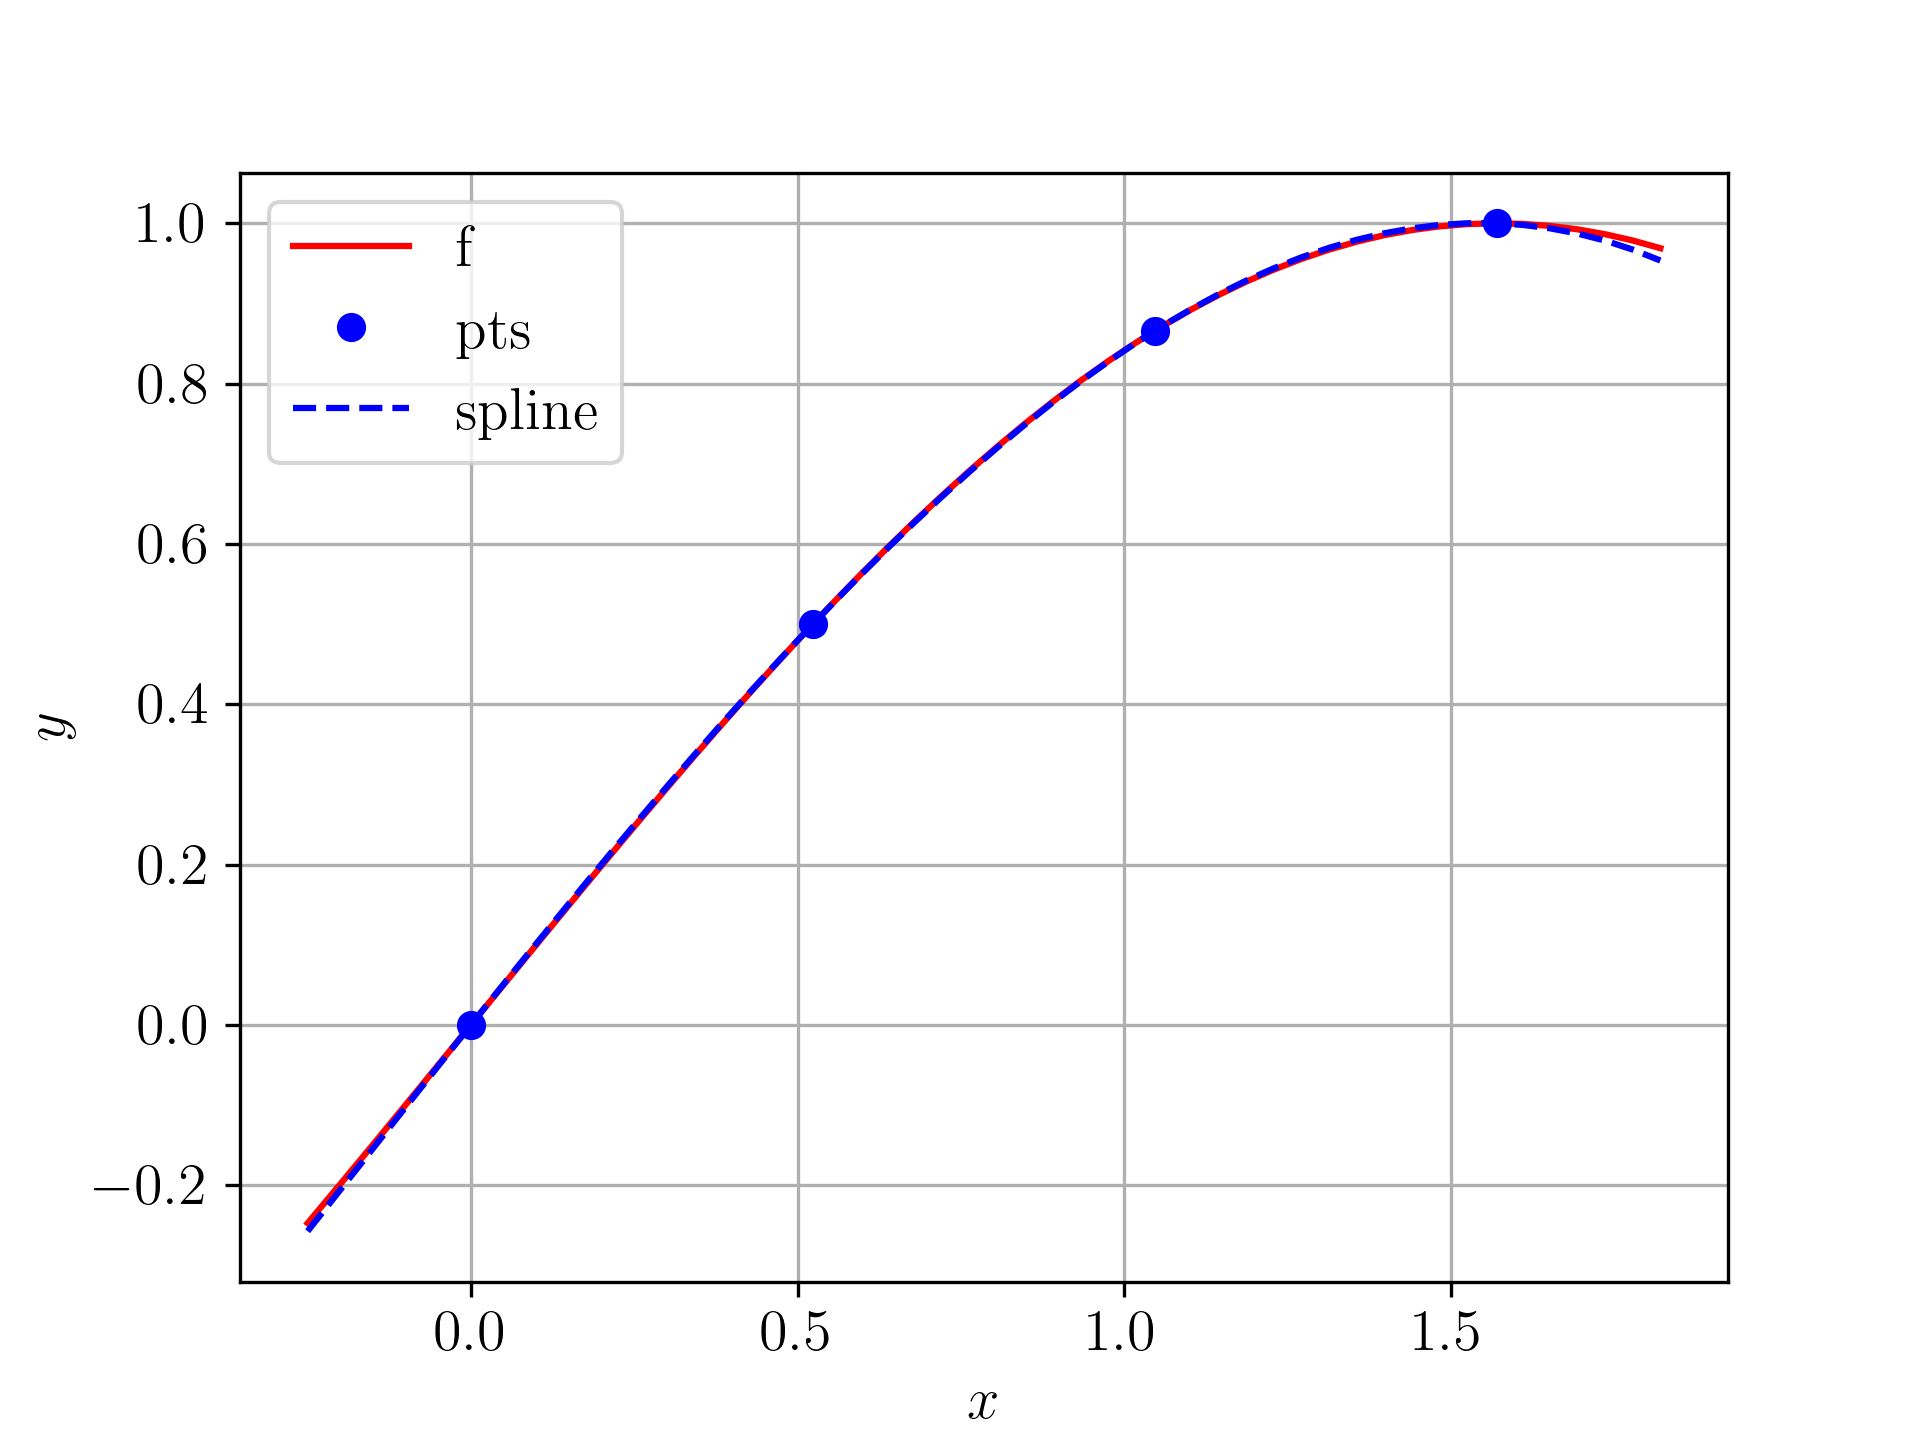
\includegraphics[width=0.8\textwidth]{./cap_interp/dados/fig_CSNotAKnot/fig}
    \caption{Esboço dos gráficos da função $f(x)=\sen(x)$ e do spline cúbico computado no Exemplo \ref{cap_interp_sec_splines:ex:interp_spline_nak}.}
    \label{cap_interp_sec_splines:fig:interp_spline_nak}
  \end{figure}

\begin{lstlisting}[caption=splineNotAKnot.py]
import numpy as np
from scipy.interpolate import CubicSpline

# dados
f = lambda x: np.sin(x)
xx = np.array([0.,
              np.pi/6,
              np.pi/3,
              np.pi/2])
yy = f(xx)

# spline
cs = CubicSpline(xx, yy)

# coefs
print(cs.c)
\end{lstlisting}
\end{ex}

\subsection{Spline Fixado}

Os \hl{splines cúbicos fixados são obtidos impondo os valores das derivadas na fronteira}, i.e.
\begin{subequations}\hleq
  \begin{align}
    &s'(x_1)=y_1',\\
    &s'(x_n)=y_n',
  \end{align}
\end{subequations}
onde $y_1'$ e $y_n'$ são escalares dados. Quando usamos splines para aproximarmos uma dada função $f$, usualmente, escolhemos $y_1'=f'(x_1)$ e $y_n'=f'(x_n)$.

\begin{ex}\label{cap_interp_sec_splines:ex:interp_spline_fixado}
  Consideremos o problema de aproximar a função $f(x)=\sen(x)$ pelo spline cúbico fixado com pontos $x_1=0$, $x_2=\pi/6$, $x_3=\pi/3$ e $x_4=\pi/2$. Na Figura \ref{cap_interp_sec_splines:fig:interp_spline_fixado} temos os esboços de $f$ e do spline cúbico computado
  \begin{equation}
    s(x) = \small\left\{
      \begin{array}{ll}
        -0.16x^3 - 0.12x^2 - 0.04x &, 0\leq x < \frac{\pi}{6}\\
        -0.001(x-\frac{\pi}{6})^3 - 0.26(x-\frac{\pi}{6})^2 - 0.44(x-\frac{\pi}{6}) + \frac{1}{2} &, \frac{\pi}{6} \leq x < \frac{\pi}{3},\\
        0.0(x-\frac{\pi}{3})^3 + 0.5(x-\frac{\pi}{3})^2 + 0.87(x-\frac{\pi}{3}) + \frac{\sqrt{3}}{2} &, \frac{\pi}{3} \leq x < \frac{\pi}{2}x
      \end{array}
\right.
  \end{equation}

  \begin{figure}[H]
    \centering
    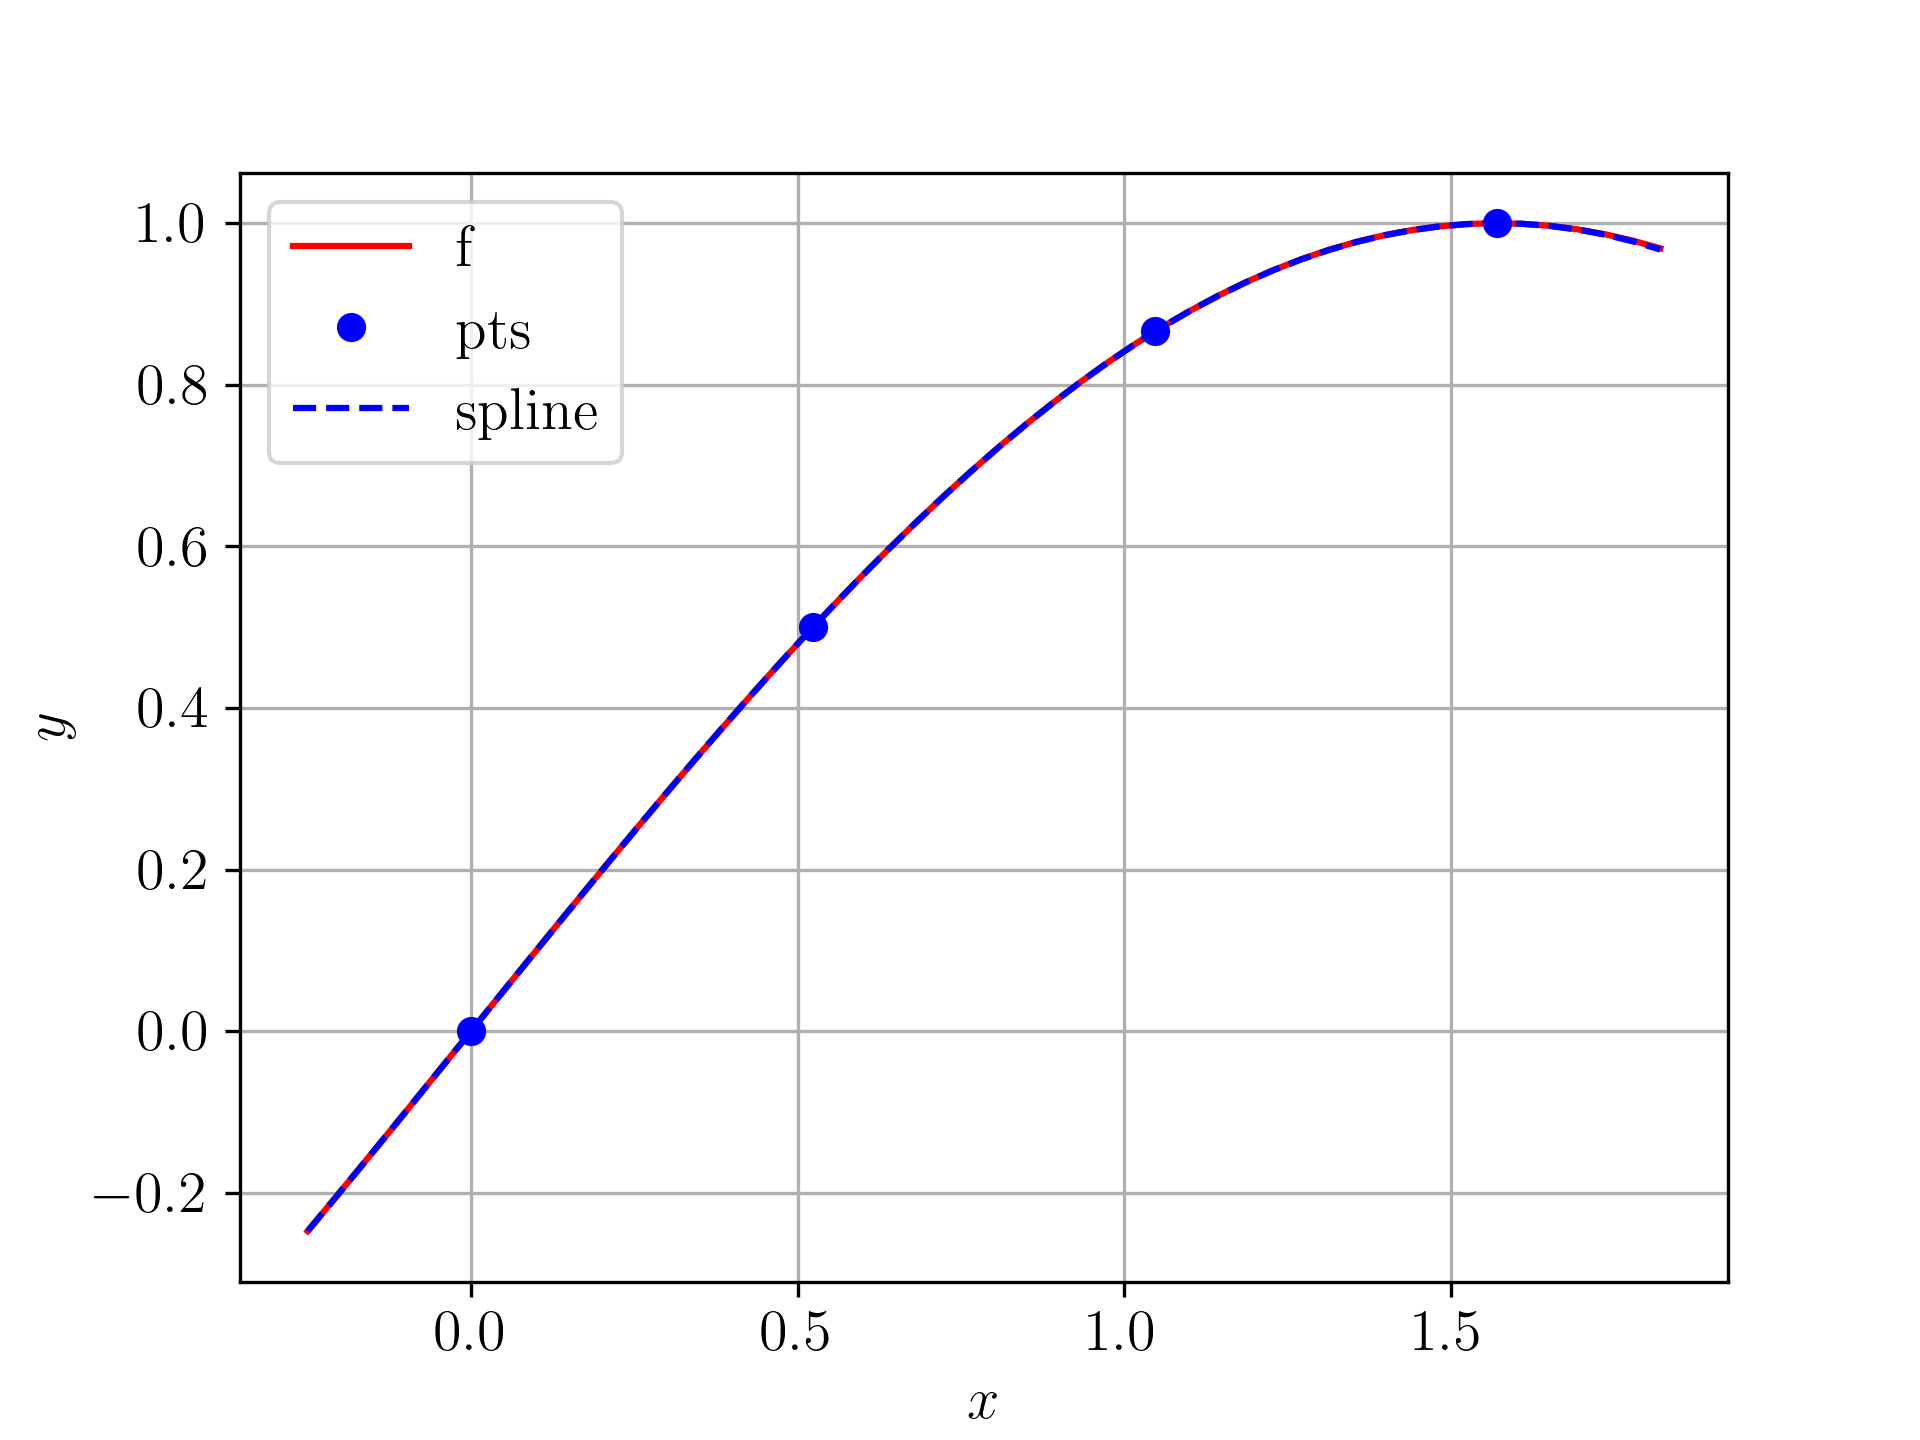
\includegraphics[width=0.8\textwidth]{./cap_interp/dados/fig_CSFixado/fig}
    \caption{Esboço dos gráficos da função $f(x)=\sen(x)$ e do spline cúbico fixado computado no Exemplo \ref{cap_interp_sec_splines:ex:interp_spline_fixado}.}
    \label{cap_interp_sec_splines:fig:interp_spline_fixado}
  \end{figure}

\begin{lstlisting}
import numpy as np
from scipy.interpolate import CubicSpline

# dados
f = lambda x: np.sin(x)
xx = np.array([0.,
              np.pi/6,
              np.pi/3,
              np.pi/2])
yy = f(xx)

# spline
cs = CubicSpline(xx, yy,
                 bc_type=((1, 1.),
                          (1, 0.)))

# coefs
print(cs.c)
\end{lstlisting}
\end{ex}

\subsection{Exercícios}

\begin{exer}
  Dado o conjunto de pontos $\{(-1, -1), (-0.5, 1), (1, 2)\}$, obtenha o spline cúbico associado com condição de controno:
  \begin{enumerate}[a)]
  \item Not-a-Knot.
  \item Fixado.
  \end{enumerate}
\end{exer}

\begin{exer}
  Dado o conjunto de pontos $\{(-1, -1), (0, 1), (1, 1/2), (2, 1)\}$, obtenha o spline cúbico associado com condição de controno:
  \begin{enumerate}[a)]
  \item Not-a-Knot.
  \item Fixado.
  \end{enumerate}
\end{exer}

\begin{exer}
  Dado o conjunto de pontos $\{(-1,~-1), (0,~1), (1,~1/2), (2,~1), (2.5, 1)\}$, obtenha o spline cúbico associado com condição de controno:
  \begin{enumerate}[a)]
  \item Not-a-Knot.
  \item Fixado.
  \end{enumerate}
\end{exer}

\begin{exer}
  Aproxime a função $f(x)=e^{x}$ por um spline cúbico que passa pelos pontos $x_1=0$, $x_2=1$, $x_3=1,5$ e $x_4=2$.
\end{exer}
\begin{resp}
  Dica: use um spline fixado.
\end{resp}

\begin{exer}
  Considere o problema de aproximar a função $f(x) = \cos(x)$ por um spline cúbico $s = s(x)$ no intervalo $[0, \pi]$. Escolha os pontos e a condição de fronteira de forma a obter $s$ que aproxime $f$ com boa precisão gráfica.
\end{exer}
\begin{resp}
  Dica: use um spline fixado.
\end{resp}
